%%%%%%%%%%%%%%%%%%%%%%%%%%%%%%%%%%%%%%%%%%%%%%%%%%
%% ICN2 pocketbook environments
%%%%%%%%%%%%%%%%%%%%%%%%%%%%%%%%%%%%%%%%%%%%%%%%%%

%%%%%%%%%%%%%%%%%%%%%%%%%%%%%%%%%%%%%%%%%%%%%%%%%%
%% Setting
%%%%%%%%%%%%%%%%%%%%%%%%%%%%%%%%%%%%%%%%%%%%%%%%%%

\newpart{part1}
\rowcolors{1}{part1!10}{white}

%\newpage
%\pagecolor{part1}
%\thispagestyle{empty}
%\mbox{}
%\newpage
%\thispagestyle{empty}
%\mbox{}
%\clearpage
%\pagecolor{white}

%% Economy %%%%%%%%%%%%%%%%%%%%%%%%%%%%%%%%%%%%%%%%%%%


\clearpage
\clearpage
\clearpage
\clearpage


\begin{ChartPage}{ Economy }
	
%   	\LeftText{\IfFileExists{./Text/TXT.P1.ECON.1.1.tex}{ECONOMY. Lorem ipsum dolor sit amet, consectetur adipiscing elit. Vestibulum lacinia faucibus libero, nec malesuada dolor volutpat vitae. Curabitur varius enim ipsum, vel lobortis metus efficitur id. Sed congue felis id tortor cursus, vitae eleifend nunc commodo. In eget molestie neque.
}{\lipsum[2]}}

% 	\RightText{\begin{chart}
% 		\caption{Value added in agriculture, industry, and services as shares of GDP}
%         		\IfFileExists{./Plots/C.P1.ECON.1.2.pdf}{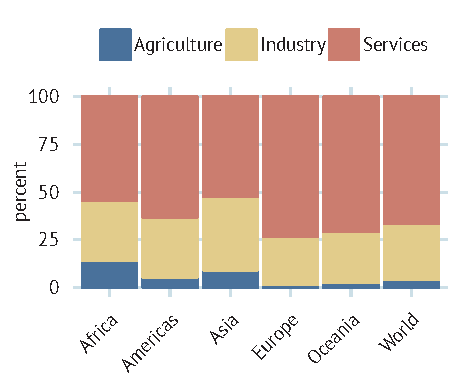
\includegraphics[width = 4cm, height = 3cm]{{./Plots/C.P1.ECON.1.2}.pdf}}{}
% 		\end{chart}}

% 	\LeftChart{\begin{chart}
% 		\caption{Agriculture value added per worker, countries with the highest values in 2013}
% 		\vspace{-7pt}
%         		\IfFileExists{./Plots/C.P1.ECON.1.3.pdf}{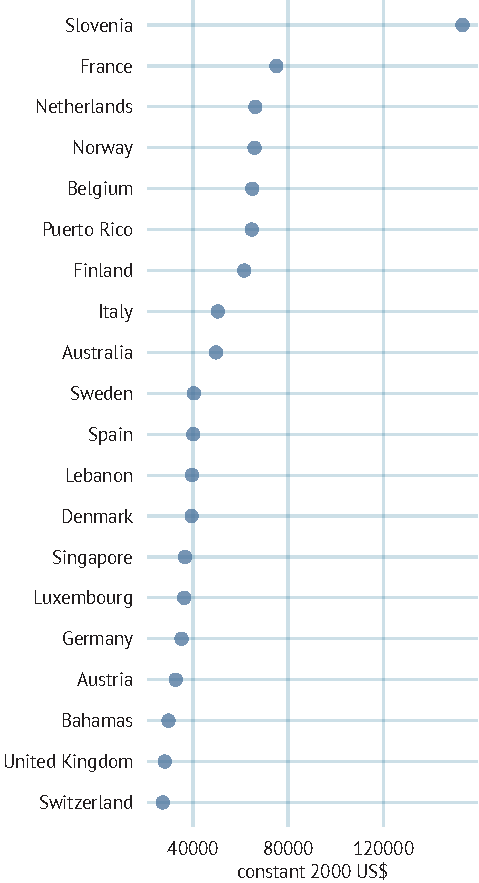
\includegraphics[width = 4cm, height = 8cm]{{./Plots/C.P1.ECON.1.3}.pdf}}{}
% 	\end{chart}} 

% 	\RightChart{\begin{chart}
% 		\caption{Value added in agriculture, average annual growth (2003-2013)}
%         		\IfFileExists{./Plots/C.P1.ECON.1.4.pdf}{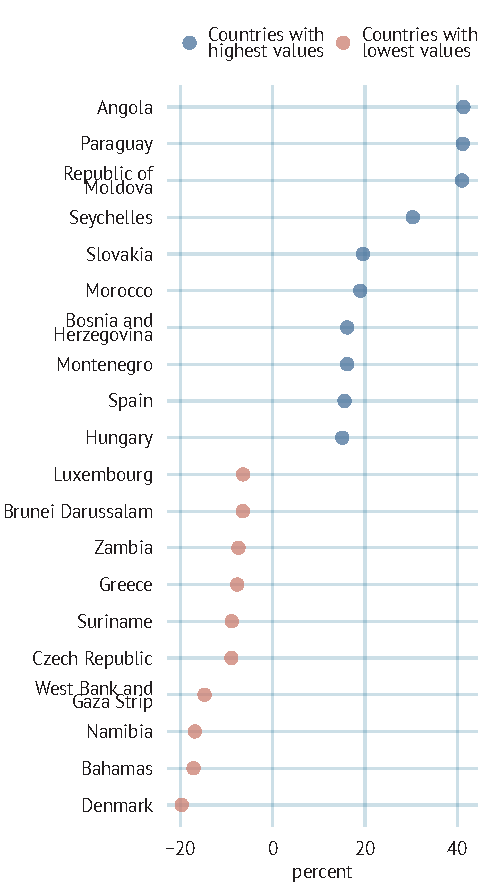
\includegraphics[width = 4cm, height = 8cm]{{./Plots/C.P1.ECON.1.4}.pdf}}{}
% 	\end{chart}} 

% 	\BottomChart{\begin{chart}
% 		\caption{Value added in agriculture as share of GDP}
% 		\IfFileExists{./Plots/C.P1.ECON.1.5.pdf}{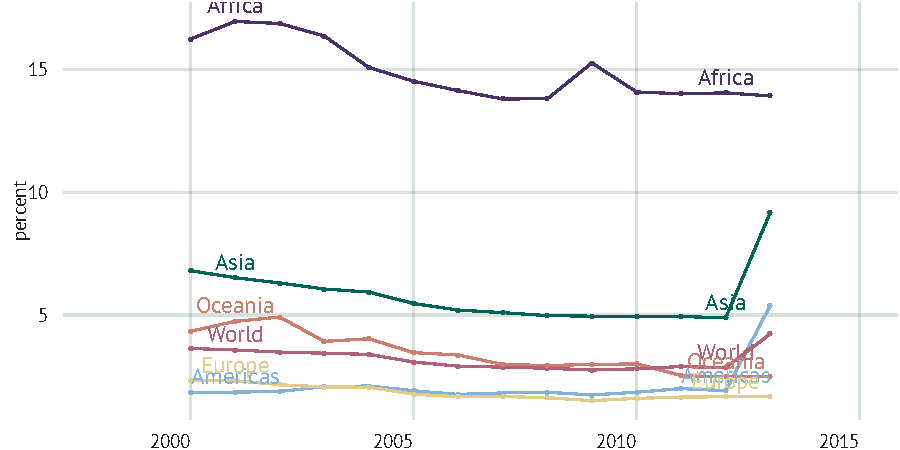
\includegraphics[width = 8cm, height = 3cm]	{{./Plots/C.P1.ECON.1.5}.pdf}}{}
% 	\end{chart}}

\end{ChartPage}

% \begin{figure}
% 	\caption{Value added in agriculture as share of GDP (percent, 2013)}
%         		\IfFileExists{./Maps/M.P1.ECON.1.6.pdf}{\centering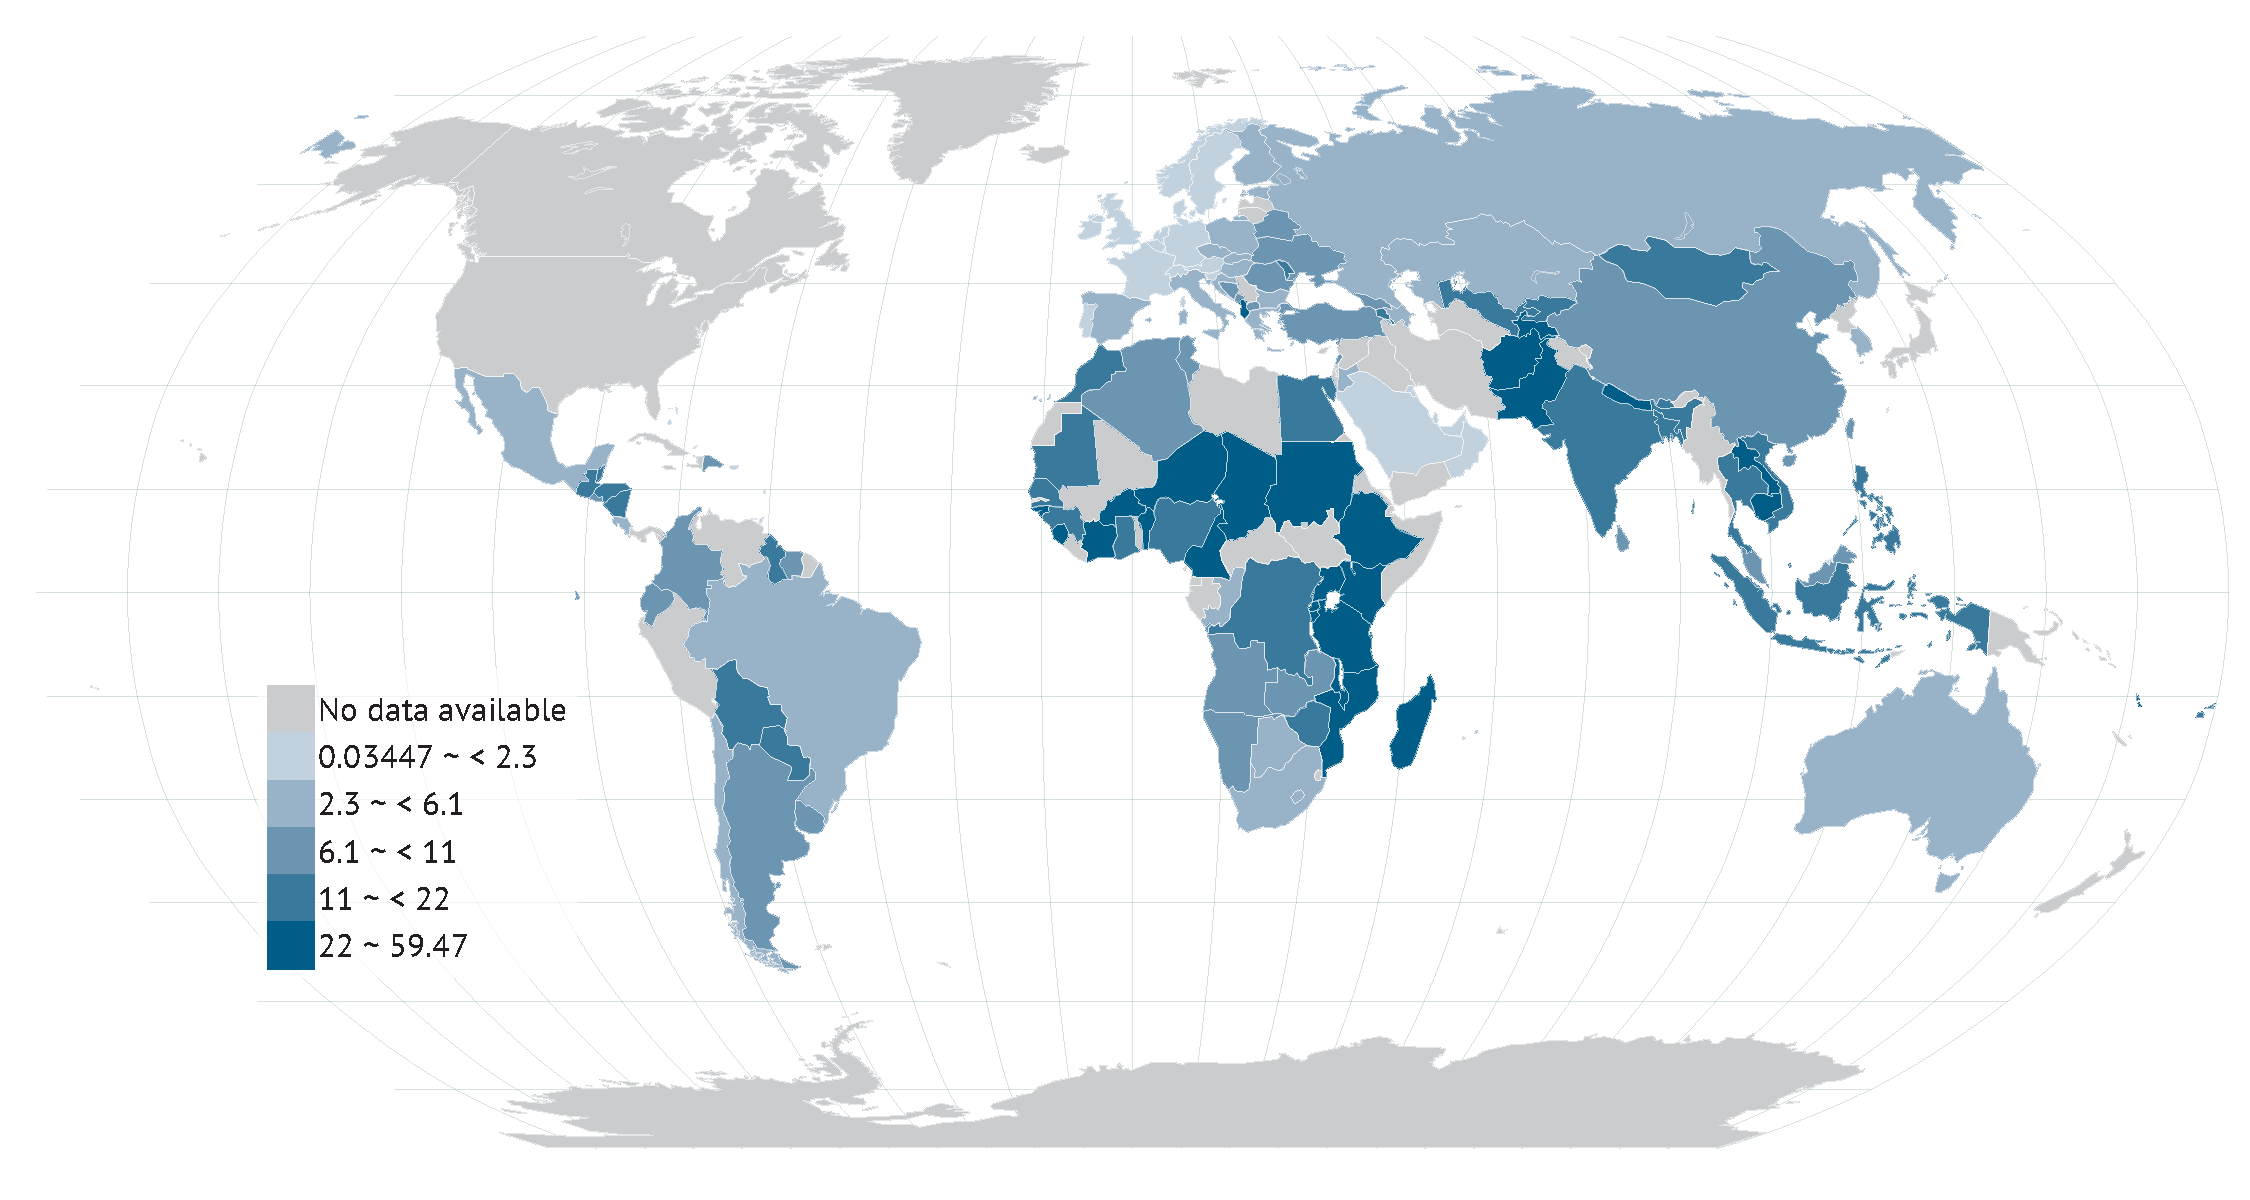
\includegraphics[height = 1\columnwidth, angle=90]{{./Maps/M.P1.ECON.1.6}.pdf}\par}{\newpage\thispagestyle{empty}\mbox{}}{}
% \end{figure}

% %% Population %%%%%%%%%%%%%%%%%%%%%%%%%%%%%%%%%%%%%%%%%%

% \begin{ChartPage}{ Population }
	
%   	\LeftText{\IfFileExists{./Text/TXT.P1.OVER.1.1.tex}{Undernourishment refers to food intake that is insufficient to meet dietary energy requirements for an active and healthy life. About 805 million people are estimated to be chronically undernourished in 2012–14. This number has fallen by 100 million over the last decade, and by 209 million since 1990-92. Despite progress, the number is still high, and marked differences across regions persist. Latin America and the Caribbean have made the greatest overall progress, with modest progress in sub-Saharan Africa and Western Asia, which have been afflicted by natural disasters and conflict.
}{\lipsum[2]}}

% %	\RightText{\IfFileExists{./Plots/MT.P1.OVER.1.2.tex}
% %		{\begin{table}
% %			\input{./Captions/Caption_MT.P1.OVER.1.2.tex}
% %			\input{./Plots/MT.P1.OVER.1.2.tex}
% %		\end{table}}}

% 	\RightText{\begin{chart}
% 		\caption{World rural and urban population (1985 to 2015)}
%         		\IfFileExists{./Plots/C.P1.OVER.1.2.pdf}{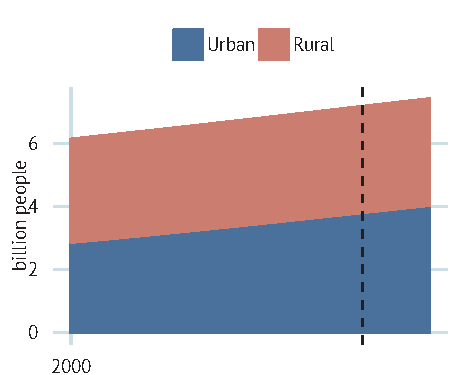
\includegraphics[width = 4cm, height = 3cm]{{./Plots/C.P1.OVER.1.2}.pdf}}{}
% 	\footnotesize{Data after 2010 are projections.}
% 		\end{chart}}

% 	\LeftChart{\begin{chart}
% 		\caption{Annual population growth over the last ten years (2004 and 2014)}
%         		\IfFileExists{./Plots/C.P1.OVER.1.3.pdf}{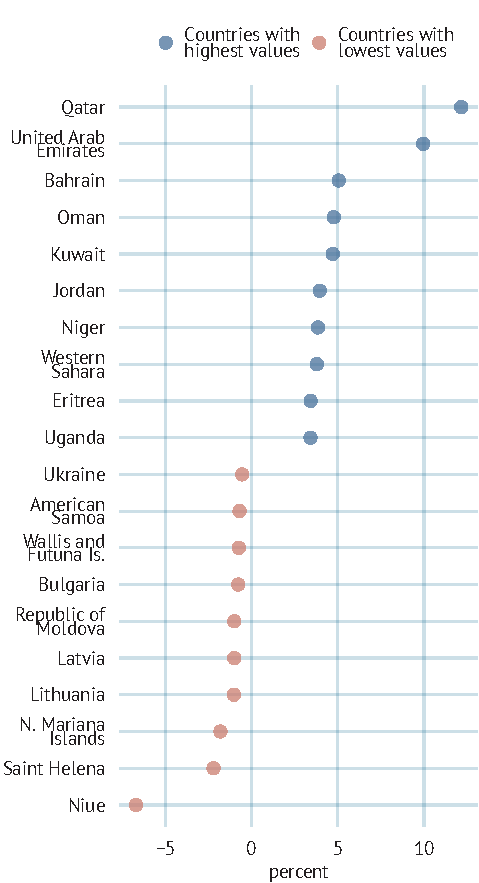
\includegraphics[width = 4cm, height = 8cm]{{./Plots/C.P1.OVER.1.3}.pdf}}{}
% 	\end{chart}} 

% 	\RightChart{\begin{chart}
% 		\caption{Life expectancy at birth, countries with the highest and lowest values (2013)}
% 		\vspace{-7pt}
%         		\IfFileExists{./Plots/C.P1.OVER.1.4.pdf}{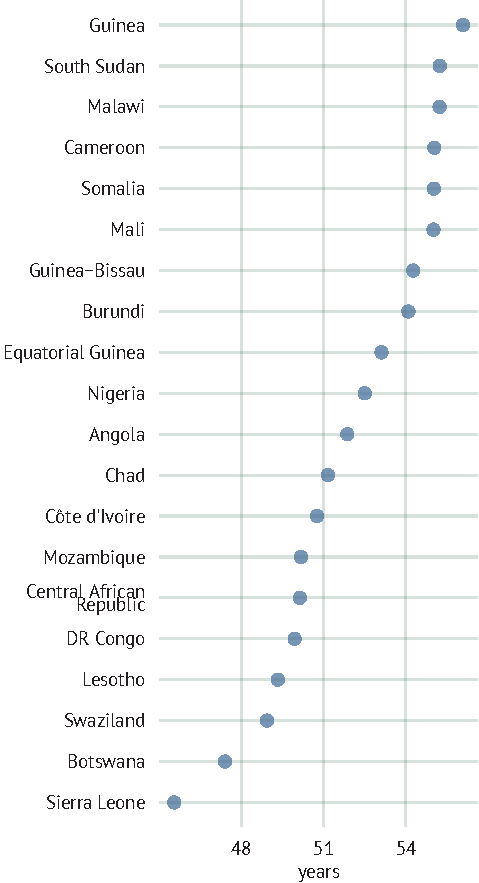
\includegraphics[width = 4cm, height = 8cm]{{./Plots/C.P1.OVER.1.4}.pdf}}{}
% 	\end{chart}} 

% 	\BottomChart{\begin{chart}
% 		\caption{Total economically active population}
% 		\IfFileExists{./Plots/C.P1.OVER.1.5.pdf}{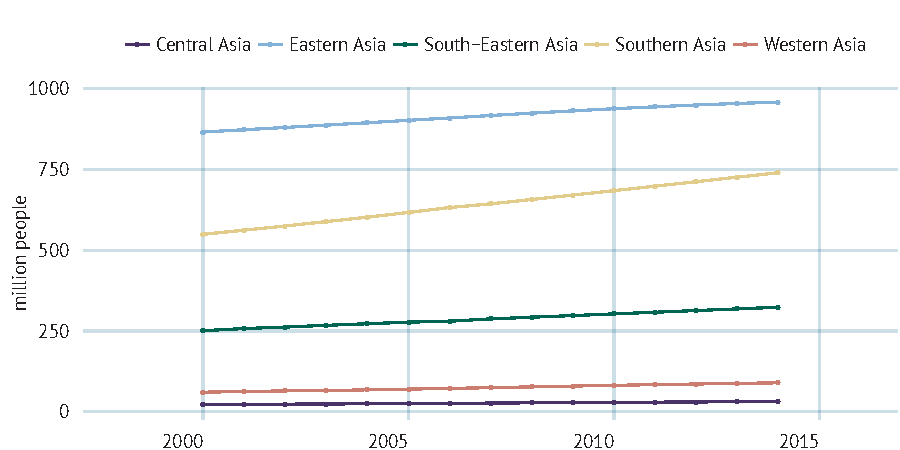
\includegraphics[width = 8cm, height = 3cm]	{{./Plots/C.P1.OVER.1.5}.pdf}}{}
% 	\end{chart}}

% \end{ChartPage}

% \begin{figure}
% 	\caption{Rural population, share of total population (percent, 2014)}
%         		\IfFileExists{./Maps/M.P1.OVER.1.6.pdf}{\centering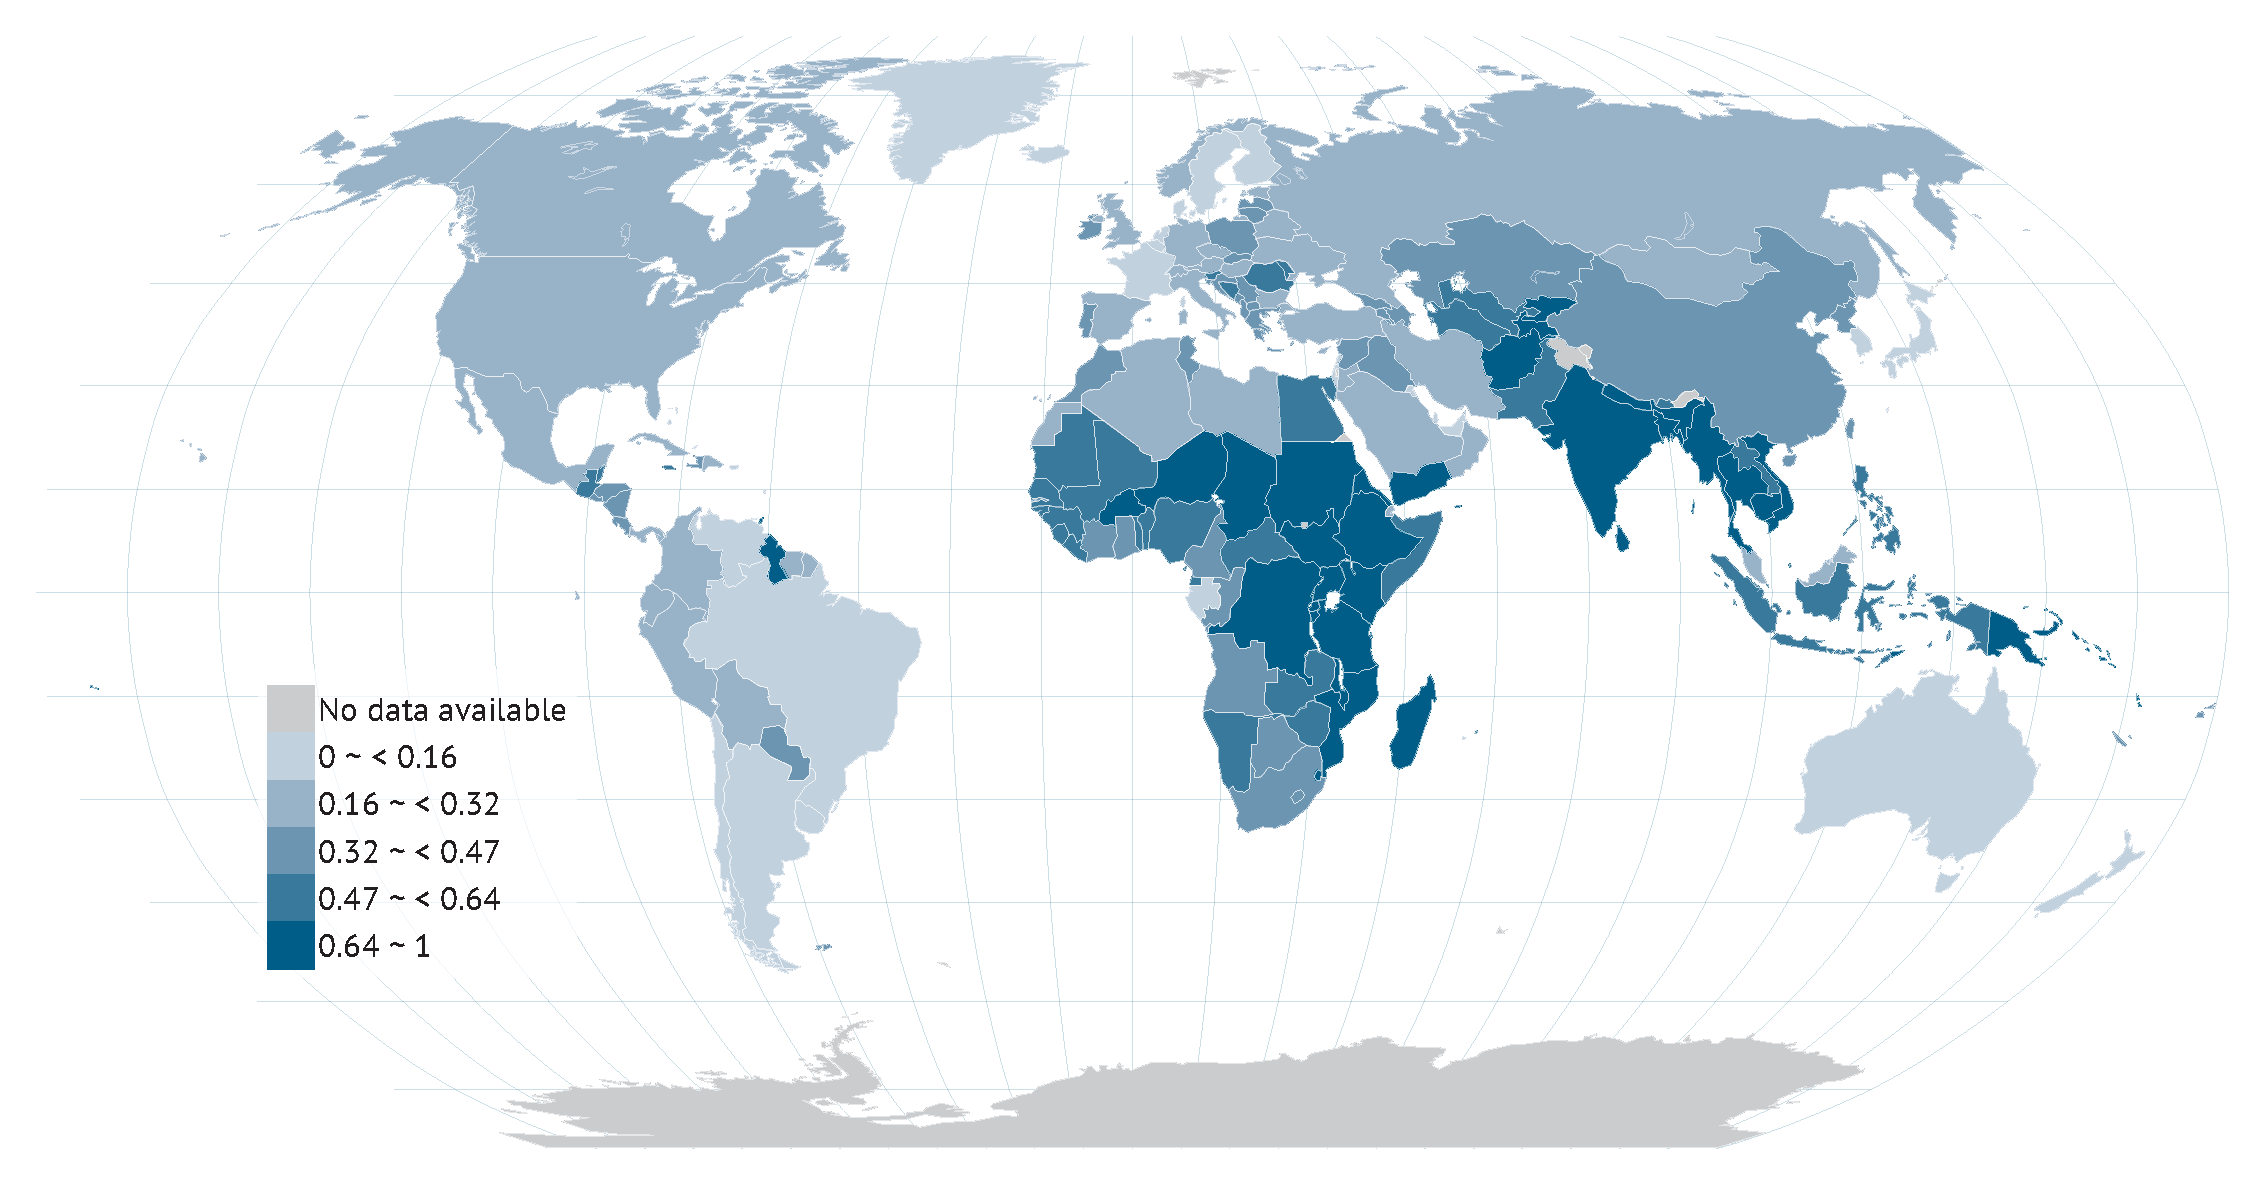
\includegraphics[height = 1\columnwidth, angle=90]{{./Maps/M.P1.OVER.1.6}.pdf}\par}{\newpage\thispagestyle{empty}\mbox{}}{}
% \end{figure}

% %% Prices %%%%%%%%%%%%%%%%%%%%%%%%%%%%%%%%%%%%%%%%%%%%%

% \begin{ChartPage}{ Prices }

%   	\LeftText{\IfFileExists{./Text/TXT.P1.PRICE.1.1.tex}{\input{./Text/TXT.P1.PRICE.1.1.tex}}{\lipsum[2]}}

% 	\RightText{\begin{chart}
% 		\input{./Captions/Caption_C.P1.PRICE.1.2.tex}
%         		\IfFileExists{./Plots/C.P1.PRICE.1.2.pdf}{\includegraphics[width = 4cm, height = 3cm]{{./Plots/C.P1.PRICE.1.2}.pdf}}{}
% 		\end{chart}}

% 	\LeftChart{\begin{chart}
% 		\input{./Captions/Caption_C.P1.PRICE.1.3.tex}
% 		\vspace{-7pt}
%         		\IfFileExists{./Plots/C.P1.PRICE.1.3.pdf}{\includegraphics[width = 4cm, height = 8cm]{{./Plots/C.P1.PRICE.1.3}.pdf}}{}
% 	\end{chart}} 

% 	\RightChart{\begin{chart}
% 		\input{./Captions/Caption_C.P1.PRICE.1.4.tex}
% 		\vspace{-7pt}
%         		\IfFileExists{./Plots/C.P1.PRICE.1.4.pdf}{\includegraphics[width = 4cm, height = 8cm]{{./Plots/C.P1.PRICE.1.4}.pdf}}{}
% 	\end{chart}} 

% 	\BottomChart{\begin{chart}
% 		\input{./Captions/Caption_C.P1.PRICE.1.5.tex}
% 		\IfFileExists{./Plots/C.P1.PRICE.1.5.pdf}{\includegraphics[width = 8cm, height = 3cm]	{{./Plots/C.P1.PRICE.1.5}.pdf}}{}
% 	\end{chart}}

% \end{ChartPage}

% \begin{figure}
% 	\input{./Captions/Caption_M.P1.PRICE.1.6.tex}
%         		\IfFileExists{./Maps/M.P1.PRICE.1.6.pdf}{\centering\includegraphics[height = 1\columnwidth, angle=90]{{./Maps/M.P1.PRICE.1.6}.pdf}\par}{\newpage\thispagestyle{empty}\mbox{}}{}
% \end{figure}

% %% Food trade %%%%%%%%%%%%%%%%%%%%%%%%%%%%%%%%%%%%%%%%%%

% \begin{ChartPage}{ Trade }

%   	\LeftText{\IfFileExists{./Text/TXT.P1.TRADE.1.1.tex}{\input{./Text/TXT.P1.TRADE.1.1.tex}}{\lipsum[2]}}

% 	\RightText{\IfFileExists{./Plots/MT.P1.TRADE.1.2.tex}
% 		{\begin{table}
% 			\input{./Captions/Caption_MT.P1.TRADE.1.2.tex}
% 			\input{./Plots/MT.P1.TRADE.1.2.tex}
% 		\end{table}}}

% 	\LeftChart{\begin{chart}
% 		\input{./Captions/Caption_C.P1.TRADE.1.3.tex}
% 		\vspace{-7pt}
%         		\IfFileExists{./Plots/C.P1.TRADE.1.3.pdf}{\includegraphics[width = 4cm, height = 8cm]{{./Plots/C.P1.TRADE.1.3}.pdf}}{}
% 	\end{chart}} 

% 	\RightChart{\begin{chart}
% 		\input{./Captions/Caption_C.P1.TRADE.1.4.tex}
% 		\vspace{-7pt}
%         		\IfFileExists{./Plots/C.P1.TRADE.1.4.pdf}{\includegraphics[width = 4cm, height = 8cm]{{./Plots/C.P1.TRADE.1.4}.pdf}}{}
% 	\end{chart}} 

% 	\BottomChart{\begin{chart}
% 		\input{./Captions/Caption_C.P1.TRADE.1.5.tex}
% 		\IfFileExists{./Plots/C.P1.TRADE.1.5.pdf}{\includegraphics[width = 8cm, height = 3cm]	{{./Plots/C.P1.TRADE.1.5}.pdf}}{}
% 	\end{chart}}

% \end{ChartPage}

% \begin{figure}
% 	\input{./Captions/Caption_M.P1.TRADE.1.6.tex}
%         		\IfFileExists{./Maps/M.P1.TRADE.1.6.pdf}{\centering\includegraphics[height = 1\columnwidth, angle=90]{{./Maps/M.P1.TRADE.1.6}.pdf}\par}{\newpage\thispagestyle{empty}\mbox{}}{}
% \end{figure}

% %%%%%%%%%%%%%%%%%%%%%%%%%%%%%%%%%%%%%%%%%%%%%%%%%%
% %% Malnutrition
% %%%%%%%%%%%%%%%%%%%%%%%%%%%%%%%%%%%%%%%%%%%%%%%%%%

% \newpart{part2}
% \rowcolors{1}{part2!10}{white}

% %\newpage
% %\pagecolor{part2}
% %\thispagestyle{empty}
% %\mbox{}
% %\newpage
% %\thispagestyle{empty}
% %\mbox{}
% %\clearpage
% %\pagecolor{white}

% %% Undernourishment %%%%%%%%%%%%%%%%%%%%%%%%%%%%%%%%%%%%%%%

% \begin{ChartPage}{ Undernourishment }

%   	\LeftText{\IfFileExists{./Text/TXT.P1.IAF.1.1.tex}{Undernourishment refers to food intake that is insufficient to meet dietary energy requirements for an active and healthy life. About 805 million people are estimated to be chronically undernourished in 2012–14. This number has fallen by 100 million over the last decade, and by 209 million since 1990-92. Despite progress, the number is still high, and marked differences across regions persist. Latin America and the Caribbean have made the greatest overall progress, with modest progress in sub-Saharan Africa and Western Asia, which have been afflicted by natural disasters and conflict.}{\lipsum[2]}}

% 	\RightText{\IfFileExists{./Plots/MT.P1.IAF.1.2.tex}
% 		{\begin{table}
% 			\caption{Prevalence of undernourishment (percent, 1990-92 and 2012-14)}
% 			\footnotesize
\begin{center}
\begin{tabular}{lrr}
\toprule
  & 1990-92 & 2012-14\\
\midrule
World & 18.7 & 11.3\\
Developing
countries & 23.4 & 13.5\\
Africa & 27.7 & 20.5\\
Asia & 23.7 & 12.7\\
Latin Am. and the Carib. & 15.3 & 6.1\\
Oceania & 15.7 & 14\\
Developed
countries & $<$5.0 & $<$5.0\\
\toprule
\end{tabular}
\end{center}

% 		\end{table}}}

% 	\LeftChart{\begin{chart}
% 		\caption{Asian countries with the highest number of people undernourished in 2012-14 (1990-92 and 2012-14)}
% 		\vspace{-7pt}
%         		\IfFileExists{./Plots/C.P1.IAF.1.3.pdf}{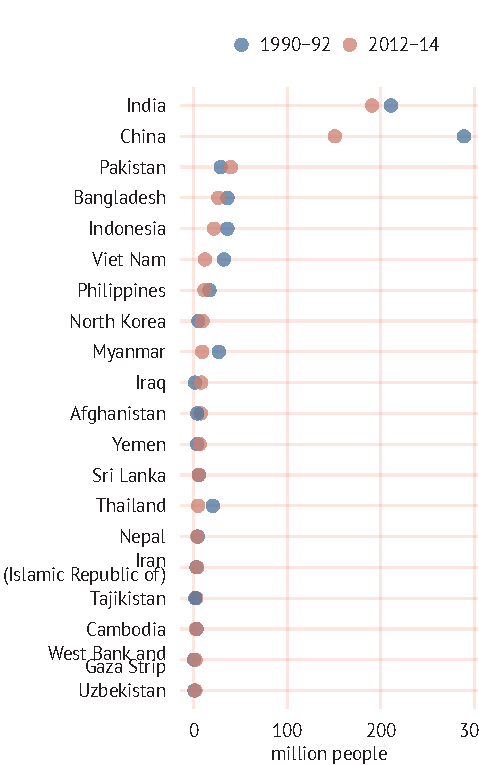
\includegraphics[width = 4cm, height = 8cm]{{./Plots/C.P1.IAF.1.3}.pdf}}{}
% 	\end{chart}} 

% 	\RightChart{\begin{chart}
% 		\caption{African countries with the highest number of people undernourished in 2012-14 (1990-92 and 2012-14)}
% 		\vspace{-7pt}
%         		\IfFileExists{./Plots/C.P1.IAF.1.4.pdf}{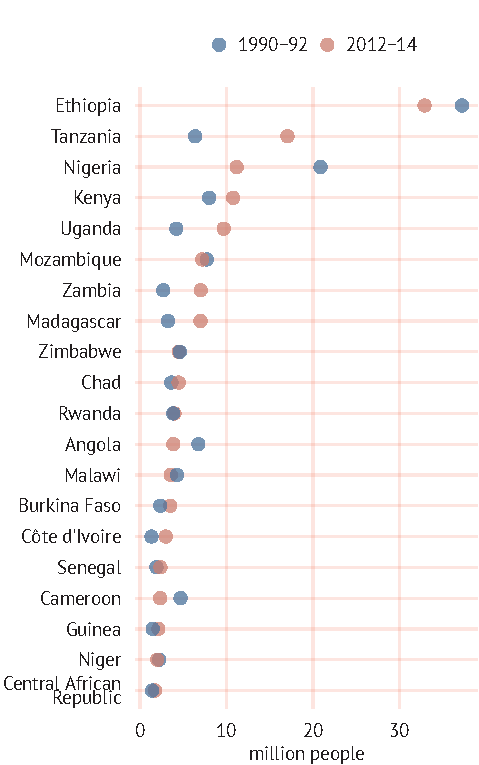
\includegraphics[width = 4cm, height = 8cm]{{./Plots/C.P1.IAF.1.4}.pdf}}{}
% 	\end{chart}} 

% 	\BottomChart{\begin{chart}
% 		\caption{Number of people undernourished (1990-92 to 2012-14)}
% 		\IfFileExists{./Plots/C.P1.IAF.1.5.pdf}{
\includegraphics[width = 8cm, height = 3cm]	{{./Plots/C.P1.IAF.1.5}.pdf}}{}
% 	\end{chart}}

% \end{ChartPage}

% \begin{figure}
% 	\caption{Prevalence of people undernourished (percent, 2014)}
%         		\IfFileExists{./Maps/M.P1.IAF.1.6.pdf}{\centering
\includegraphics[height = 1\columnwidth, angle=90]{{./Maps/M.P1.IAF.1.6}.pdf}\par}{\newpage\thispagestyle{empty}\mbox{}}{}
% \end{figure}

% %% Undernutrition %%%%%%%%%%%%%%%%%%%%%%%%%%%%%%%%%%%%%%%%%

% \begin{Chart2Page}{ Undernutrition }
	
%   	\LeftText{\IfFileExists{./Text/TXT.P1.UT.1.1.tex}{\input{./Text/TXT.P1.UT.1.1.tex}}{\lipsum[2]}}

% 	\RightText{\IfFileExists{./Plots/MT.P1.UT.1.2}
% 		{\begin{table}
% 			\input{./Captions/Caption_MT.P1.UT.1.2.tex}
% 			\input{./Plots/MT.P1.UT.1.2.tex}
% 		\end{table}}}

% 	\LeftChart{\begin{chart}
% 		\input{./Captions/Caption_C.P1.UT.1.3.tex}
%         		\IfFileExists{./Plots/C.P1.UT.1.3.pdf}{\includegraphics[width = 4cm, height = 8cm]{{./Plots/C.P1.UT.1.3}.pdf}}{}
% 	\end{chart}} 

% 	\RightChart{\begin{chart}
% 		\input{./Captions/Caption_C.P1.UT.1.4.tex}
%         		\IfFileExists{./Plots/C.P1.UT.1.4.pdf}{\includegraphics[width = 4cm, height = 8cm]{{./Plots/C.P1.UT.1.4}.pdf}}{}
% 	\end{chart}} 
          
% 	\BottomLeftChart{\IfFileExists{./Plots/MT.P1.UT.1.5}
% 		{\begin{table}
% 			\input{./Captions/Caption_MT.P1.UT.1.5.tex}
% 			\input{./Plots/MT.P1.UT.1.5.tex}
% 		\end{table}}}

% 	\BottomRightChart{\IfFileExists{./Plots/MT.P1.UT.1.6}
% 		{\begin{table}
% 			\input{./Captions/Caption_MT.P1.UT.1.6.tex}
% 			\input{./Plots/MT.P1.UT.1.6.tex}
% 		\end{table}}}

% \end{Chart2Page}

% \begin{figure}
% 	\input{./Captions/Caption_M.P1.UT.1.7.tex}
%         		\IfFileExists{./Maps/M.P1.UT.1.7.pdf}{\centering\includegraphics[height = 1\columnwidth, angle=90]{{./Maps/M.P1.UT.1.7}.pdf}\par}{\newpage\thispagestyle{empty}\mbox{}}{}
% \end{figure}

% %% Obesity/Overweight %%%%%%%%%%%%%%%%%%%%%%%%%%%%%%%%%%%%%%

% \begin{ChartPage}{ Overweight/Obesity }

%   	\LeftText{\IfFileExists{./Text/TXT.P1.OO.1.1.tex}{\input{./Text/TXT.P1.OO.1.1.tex}}{\lipsum[2]}}

% 	\RightText{\begin{chart}
% 		\input{./Captions/Caption_C.P1.OO.1.2.tex}
%         		\IfFileExists{./Plots/C.P1.OO.1.2.pdf}{\includegraphics[width = 4cm, height = 3cm]{{./Plots/C.P1.OO.1.2}.pdf}}{}
% 		\end{chart}}

% 	\LeftChart{\begin{chart}
% 		\input{./Captions/Caption_C.P1.OO.1.3.tex}
%         		\IfFileExists{./Plots/C.P1.OO.1.3.pdf}{\includegraphics[width = 4cm, height = 8cm]{{./Plots/C.P1.OO.1.3}.pdf}}{}
% 	\end{chart}} 

% 	\RightChart{\begin{chart}
% 		\input{./Captions/Caption_C.P1.OO.1.4.tex}
%         		\IfFileExists{./Plots/C.P1.OO.1.4.pdf}{\includegraphics[width = 4cm, height = 8cm]{{./Plots/C.P1.OO.1.4}.pdf}}{}
% 	\end{chart}} 

% 	\BottomChart{\begin{chart}
% 		\input{./Captions/Caption_C.P1.OO.1.5.tex}
% 		\IfFileExists{./Plots/C.P1.OO.1.5.pdf}{\includegraphics[width = 8cm, height = 3cm]	{{./Plots/C.P1.OO.1.5}.pdf}}{}
% 	\end{chart}}

% \end{ChartPage}

% \begin{figure}
% 	\input{./Captions/Caption_M.P1.OO.1.6.tex}
%         		\IfFileExists{./Maps/M.P1.OO.1.6.pdf}{\centering\includegraphics[height = 1\columnwidth, angle=90]{{./Maps/M.P1.OO.1.6}.pdf}\par}{\newpage\thispagestyle{empty}\mbox{}}{}
% \end{figure}

% %%  Food security indicators %%%%%%%%%%%%%%%%%%%%%%%%%%%%%%%%%%%%

% \begin{ChartPage}{ Food security indicators }

%   	\LeftText{\IfFileExists{./Text/TXT.P1.FSI.1.1.tex}{\input{./Text/TXT.P1.FSI.1.1.tex}}{\lipsum[8]}}
%   	\RightText{\IfFileExists{./Text/TXT.P1.FSI.1.2.tex}{\input{./Text/TXT.P1.FSI.1.2.tex}}{\lipsum[8]}}

% 	\LeftChart{
%            	\centering
% 		\includegraphics[width = 8cm]{./FSIindicators.png}
% 	} 
	
% 	\RightChart{

% 	}	
% 	\BottomChart{
% %	\justify
% %	\lipsum[8]
% 	\clearpage
% 	}
% \end{ChartPage}

% \begin{multicols}{2}

% 	\includegraphics[width = 3.8cm]{./SOFI_1.png}
% 	\includegraphics[width = 3.8cm]{./SOFI_2.png}
% 	\includegraphics[width = 3.8cm]{./SOFI_3.png}
% 	\includegraphics[width = 3.8cm]{./SOFI_4.png}
% 	\includegraphics[width = 3.8cm]{./SOFI_5.png}
% 	\includegraphics[width = 3.8cm]{./SOFI_6.png}
% 	\includegraphics[width = 3.8cm]{./SOFI_7.png}
% 	\includegraphics[width = 3.8cm]{./SOFI_8.png}
% 	\includegraphics[width = 3.8cm]{./SOFI_9.png}
% 	\includegraphics[width = 3.8cm]{./SOFI_all_regions.png}
% 	\includegraphics[width = 3.8cm]{./SOFI_key.png}
% \end{multicols}

% %%%%%%%%%%%%%%%%%%%%%%%%%%%%%%%%%%%%%%%%%%%%%%%%%%
% %% Diets
% %%%%%%%%%%%%%%%%%%%%%%%%%%%%%%%%%%%%%%%%%%%%%%%%%%

% \newpart{part3}
% \rowcolors{1}{part3!10}{white}

% %\newpage
% %\pagecolor{part3}
% %\thispagestyle{empty}
% %\mbox{}
% %\newpage
% %\thispagestyle{empty}
% %\mbox{}
% %\clearpage
% %\pagecolor{white}

% %% Dietary energy supply %%%%%%%%%%%%%%%%%%%%%%%%%%%%%%%%%%%%%%

% \begin{ChartPage}{ Dietary energy supply }
	
%   	\LeftText{\IfFileExists{./Text/TXT.P1.DES.1.1.tex}{\input{./Text/TXT.P1.DES.1.1.tex}}{\lipsum[2]}}

% 	\RightText{\begin{chart}
% 		\input{./Captions/Caption_C.P1.DES.1.2.tex}
%         		\IfFileExists{./Plots/C.P1.DES.1.2.pdf}{\includegraphics[width = 4cm, height = 3cm]{{./Plots/C.P1.DES.1.2}.pdf}}{}
% 		\end{chart}}

% 	\LeftChart{\begin{chart}
% 		\input{./Captions/Caption_C.P1.DES.1.3.tex}
% 		\vspace{-7pt}
%         		\IfFileExists{./Plots/C.P1.DES.1.3.pdf}{\includegraphics[width = 4cm, height = 8cm]{{./Plots/C.P1.DES.1.3}.pdf}}{}
% 	\end{chart}} 

% 	\RightChart{\begin{chart}
% 		\input{./Captions/Caption_C.P1.DES.1.4.tex}
% 		\vspace{-7pt}
%         		\IfFileExists{./Plots/C.P1.DES.1.4.pdf}{\includegraphics[width = 4cm, height = 8cm]{{./Plots/C.P1.DES.1.4}.pdf}}{}
% 	\end{chart}} 

% 	\BottomChart{\begin{chart}
% 		\input{./Captions/Caption_C.P1.DES.1.5.tex}
% 		\IfFileExists{./Plots/C.P1.DES.1.5.pdf}{\includegraphics[width = 8cm, height = 3cm]	{{./Plots/C.P1.DES.1.5}.pdf}}{}
% 	\end{chart}}

% \end{ChartPage}

% \begin{figure}
% 	\input{./Captions/Caption_M.P1.DES.1.6.tex}
%         		\IfFileExists{./Maps/M.P1.DES.1.6.pdf}{\centering\includegraphics[height = 1\columnwidth, angle=90]{{./Maps/M.P1.DES.1.6}.pdf}\par}{\newpage\thispagestyle{empty}\mbox{}}{}
% \end{figure}

% %% Cereals %%%%%%%%%%%%%%%%%%%%%%%%%%%%%%%%%%%%%%%%%%%%

% \begin{ChartPage}{ Cereals - excluding beer }
	
%   	\LeftText{\IfFileExists{./Text/TXT.P1.CRLS.1.1.tex}{\input{./Text/TXT.P1.CRLS.1.1.tex}}{\lipsum[2]}}

% 	\RightText{\begin{chart}
% 		\input{./Captions/Caption_C.P1.CRLS.1.2.tex}
%         		\IfFileExists{./Plots/C.P1.CRLS.1.2.pdf}{\includegraphics[width = 4cm, height = 3cm]{{./Plots/C.P1.CRLS.1.2}.pdf}}{}
% 		\end{chart}}

% 	\LeftChart{\begin{chart}
% 		\input{./Captions/Caption_C.P1.CRLS.1.3.tex}
% 		\vspace{-7pt}
%         		\IfFileExists{./Plots/C.P1.CRLS.1.3.pdf}{\includegraphics[width = 4cm, height = 8cm]{{./Plots/C.P1.CRLS.1.3}.pdf}}{}
% 	\end{chart}} 

% 	\RightChart{\begin{chart}
% 		\input{./Captions/Caption_C.P1.CRLS.1.4.tex}
% 		\vspace{-7pt}
%         		\IfFileExists{./Plots/C.P1.CRLS.1.4.pdf}{\includegraphics[width = 4cm, height = 8cm]{{./Plots/C.P1.CRLS.1.4}.pdf}}{}
% 	\end{chart}} 

% 	\BottomChart{\begin{chart}
% 		\input{./Captions/Caption_C.P1.CRLS.1.5.tex}
% 		\IfFileExists{./Plots/C.P1.CRLS.1.5.pdf}{\includegraphics[width = 8cm, height = 3cm]	{{./Plots/C.P1.CRLS.1.5}.pdf}}{}
% 	\end{chart}}

% \end{ChartPage}

% \begin{figure}
% 	\input{./Captions/Caption_M.P1.CRLS.1.6.tex}
%         		\IfFileExists{./Maps/M.P1.CRLS.1.6.pdf}{\centering\includegraphics[height = 1\columnwidth, angle=90]{{./Maps/M.P1.CRLS.1.6}.pdf}\par}{\newpage\thispagestyle{empty}\mbox{}}{}
% \end{figure}

% %% Starchy roots %%%%%%%%%%%%%%%%%%%%%%%%%%%%%%%%%%%%%%%%%

% \begin{ChartPage}{ Starchy roots }

%   	\LeftText{\IfFileExists{./Text/TXT.P1.SR.1.1.tex}{\input{./Text/TXT.P1.SR.1.1.tex}}{\lipsum[2]}}

% 	\RightText{\begin{chart}
% 		\input{./Captions/Caption_C.P1.SR.1.2.tex}
%         		\IfFileExists{./Plots/C.P1.SR.1.2.pdf}{\includegraphics[width = 4cm, height = 3cm]{{./Plots/C.P1.SR.1.2}.pdf}}{}
% 		\end{chart}}

% 	\LeftChart{\begin{chart}
% 		\input{./Captions/Caption_C.P1.SR.1.3.tex}
% %		\vspace{-7pt}
%         		\IfFileExists{./Plots/C.P1.SR.1.3.pdf}{\includegraphics[width = 4cm, height = 8cm]{{./Plots/C.P1.SR.1.3}.pdf}}{}
% 	\end{chart}} 

% 	\RightChart{\begin{chart}
% 		\input{./Captions/Caption_C.P1.SR.1.4.tex}
% 		\vspace{-7pt}
%         		\IfFileExists{./Plots/C.P1.SR.1.4.pdf}{\includegraphics[width = 4cm, height = 8cm]{{./Plots/C.P1.SR.1.4}.pdf}}{}
% 	\end{chart}} 

% 	\BottomChart{\begin{chart}
% 		\input{./Captions/Caption_C.P1.SR.1.5.tex}
% 		\IfFileExists{./Plots/C.P1.SR.1.5.pdf}{\includegraphics[width = 8cm, height = 3cm]	{{./Plots/C.P1.SR.1.5}.pdf}}{}
% 	\end{chart}}

% \end{ChartPage}

% \begin{figure}
% 	\input{./Captions/Caption_M.P1.SR.1.6.tex}
%         		\IfFileExists{./Maps/M.P1.SR.1.6.pdf}{\centering\includegraphics[height = 1\columnwidth, angle=90]{{./Maps/M.P1.SR.1.6}.pdf}\par}{\newpage\thispagestyle{empty}\mbox{}}{}
% \end{figure}


% %% Sugar and sweeteners %%%%%%%%%%%%%%%%%%%%%%%%%%%%%%%%%%%%%

% \begin{ChartPage}{ Sugar and sweeteners }

%   	\LeftText{\IfFileExists{./Text/TXT.P1.SS.1.1.tex}{\input{./Text/TXT.P1.SS.1.1.tex}}{\lipsum[2]}}

% 	\RightText{\begin{chart}
% 		\input{./Captions/Caption_C.P1.SS.1.2.tex}
%         		\IfFileExists{./Plots/C.P1.SS.1.2.pdf}{\includegraphics[width = 4cm, height = 3cm]{{./Plots/C.P1.SS.1.2}.pdf}}{}
% 		\end{chart}}

% 	\LeftChart{\begin{chart}
% 		\input{./Captions/Caption_C.P1.SS.1.3.tex}
% 		\vspace{-7pt}
%         		\IfFileExists{./Plots/C.P1.SS.1.3.pdf}{\includegraphics[width = 4cm, height = 8cm]{{./Plots/C.P1.SS.1.3}.pdf}}{}
% 	\end{chart}} 

% 	\RightChart{\begin{chart}
% 		\input{./Captions/Caption_C.P1.SS.1.4.tex}
% 		\vspace{-7pt}
%         		\IfFileExists{./Plots/C.P1.SS.1.4.pdf}{\includegraphics[width = 4cm, height = 8cm]{{./Plots/C.P1.SS.1.4}.pdf}}{}
% 	\end{chart}} 

% 	\BottomChart{\begin{chart}
% 		\input{./Captions/Caption_C.P1.SS.1.5.tex}
% 		\IfFileExists{./Plots/C.P1.SS.1.5.pdf}{\includegraphics[width = 8cm, height = 3cm]	{{./Plots/C.P1.SS.1.5}.pdf}}{}
% 	\end{chart}}

% \end{ChartPage}

% \begin{figure}
% 	\input{./Captions/Caption_M.P1.SS.1.6.tex}
%         		\IfFileExists{./Maps/M.P1.SS.1.6.pdf}{\centering\includegraphics[height = 1\columnwidth, angle=90]{{./Maps/M.P1.SS.1.6}.pdf}\par}{\newpage\thispagestyle{empty}\mbox{}}{}
% \end{figure}

% %% Fruit and Vegetable %%%%%%%%%%%%%%%%%%%%%%%%%%%%%%%%%%%%%%%%%

% \begin{ChartPage}{ Fruit and vegetables }

%   	\LeftText{\IfFileExists{./Text/TXT.P1.FV.1.1.tex}{\input{./Text/TXT.P1.FV.1.1.tex}}{\lipsum[2]}}

% 	\RightText{\begin{chart}
% 		\input{./Captions/Caption_C.P1.FV.1.2.tex}
%         		\IfFileExists{./Plots/C.P1.FV.1.2.pdf}{\includegraphics[width = 4cm, height = 3cm]{{./Plots/C.P1.FV.1.2}.pdf}}{}
% 		\end{chart}}

% 	\LeftChart{\begin{chart}
% 		\input{./Captions/Caption_C.P1.FV.1.3.tex}
% 		\vspace{-7pt}
%         		\IfFileExists{./Plots/C.P1.FV.1.3.pdf}{\includegraphics[width = 4cm, height = 8cm]{{./Plots/C.P1.FV.1.3}.pdf}}{}
% 	\end{chart}} 

% 	\RightChart{\begin{chart}
% 		\input{./Captions/Caption_C.P1.FV.1.4.tex}
% 		\vspace{-7pt}
%         		\IfFileExists{./Plots/C.P1.FV.1.4.pdf}{\includegraphics[width = 4cm, height = 8cm]{{./Plots/C.P1.FV.1.4}.pdf}}{}
% 	\end{chart}} 

% 	\BottomChart{\begin{chart}
% 		\input{./Captions/Caption_C.P1.FV.1.5.tex}
% 		\IfFileExists{./Plots/C.P1.FV.1.5.pdf}{\includegraphics[width = 8cm, height = 3cm]	{{./Plots/C.P1.FV.1.5}.pdf}}{}
% 	\end{chart}}

% \end{ChartPage}

% \begin{figure}
% 	\input{./Captions/Caption_M.P1.FV.1.6.tex}
%         		\IfFileExists{./Maps/M.P1.FV.1.6.pdf}{\centering\includegraphics[height = 1\columnwidth, angle=90]{{./Maps/M.P1.FV.1.6}.pdf}\par}{\newpage\thispagestyle{empty}\mbox{}}{}
% \end{figure}

% %% Meat %%%%%%%%%%%%%%%%%%%%%%%%%%%%%%%%%%%%%%%%%%%%

% \begin{ChartPage}{ Meat }

%   	\LeftText{\IfFileExists{./Text/TXT.P1.MEAT.1.1.tex}{\input{./Text/TXT.P1.MEAT.1.1.tex}}{\lipsum[2]}}

% 	\RightText{\begin{chart}
% 		\input{./Captions/Caption_C.P1.MEAT.1.2.tex}
%         		\IfFileExists{./Plots/C.P1.MEAT.1.2.pdf}{\includegraphics[width = 4cm, height = 3cm]{{./Plots/C.P1.MEAT.1.2}.pdf}}{}
% 		\end{chart}}

% 	\LeftChart{\begin{chart}
% 		\input{./Captions/Caption_C.P1.MEAT.1.3.tex}
% 		\vspace{-7pt}
%         		\IfFileExists{./Plots/C.P1.MEAT.1.3.pdf}{\includegraphics[width = 4cm, height = 8cm]{{./Plots/C.P1.MEAT.1.3}.pdf}}{}
% 	\end{chart}} 

% 	\RightChart{\begin{chart}
% 		\input{./Captions/Caption_C.P1.MEAT.1.4.tex}
% 		\vspace{-7pt}
%         		\IfFileExists{./Plots/C.P1.MEAT.1.4.pdf}{\includegraphics[width = 4cm, height = 8cm]{{./Plots/C.P1.MEAT.1.4}.pdf}}{}
% 	\end{chart}} 

% 	\BottomChart{\begin{chart}
% 		\input{./Captions/Caption_C.P1.MEAT.1.5.tex}
% 		\IfFileExists{./Plots/C.P1.MEAT.1.5.pdf}{\includegraphics[width = 8cm, height = 3cm]	{{./Plots/C.P1.MEAT.1.5}.pdf}}{}
% 	\end{chart}}

% \end{ChartPage}

% \begin{figure}
% 	\input{./Captions/Caption_M.P1.MEAT.1.6.tex}
%         		\IfFileExists{./Maps/M.P1.MEAT.1.6.pdf}{\centering\includegraphics[height = 1\columnwidth, angle=90]{{./Maps/M.P1.MEAT.1.6}.pdf}\par}{\newpage\thispagestyle{empty}\mbox{}}{}
% \end{figure}

% %% Oilcrops %%%%%%%%%%%%%%%%%%%%%%%%%%%%%%%%%%%%%%%%%%%

% \begin{ChartPage}{ Oilcrops }

%   	\LeftText{\IfFileExists{./Text/TXT.P1.OCRPS.1.1.tex}{\input{./Text/TXT.P1.OCRPS.1.1.tex}}{\lipsum[2]}}

% 	\RightText{\begin{chart}
% 		\input{./Captions/Caption_C.P1.OCRPS.1.2.tex}
%         		\IfFileExists{./Plots/C.P1.OCRPS.1.2.pdf}{\includegraphics[width = 4cm, height = 3cm]{{./Plots/C.P1.OCRPS.1.2}.pdf}}{}
% 		\end{chart}}

% 	\LeftChart{\begin{chart}
% 		\input{./Captions/Caption_C.P1.OCRPS.1.3.tex}
% 		\vspace{-7pt}
%         		\IfFileExists{./Plots/C.P1.OCRPS.1.3.pdf}{\includegraphics[width = 4cm, height = 8cm]{{./Plots/C.P1.OCRPS.1.3}.pdf}}{}
% 	\end{chart}} 

% 	\RightChart{\begin{chart}
% 		\input{./Captions/Caption_C.P1.OCRPS.1.4.tex}
% 		\vspace{-7pt}
%         		\IfFileExists{./Plots/C.P1.OCRPS.1.4.pdf}{\includegraphics[width = 4cm, height = 8cm]{{./Plots/C.P1.OCRPS.1.4}.pdf}}{}
% 	\end{chart}} 

% 	\BottomChart{\begin{chart}
% 		\input{./Captions/Caption_C.P1.OCRPS.1.5.tex}
% 		\IfFileExists{./Plots/C.P1.OCRPS.1.5.pdf}{\includegraphics[width = 8cm, height = 3cm]	{{./Plots/C.P1.OCRPS.1.5}.pdf}}{}
% 	\end{chart}}

% \end{ChartPage}

% \begin{figure}
% 	\input{./Captions/Caption_M.P1.OCRPS.1.6.tex}
%         		\IfFileExists{./Maps/M.P1.OCRPS.1.6.pdf}{\centering\includegraphics[height = 1\columnwidth, angle=90]{{./Maps/M.P1.OCRPS.1.6}.pdf}\par}{\newpage\thispagestyle{empty}\mbox{}}{}
% \end{figure}

% %% Fish %%%%%%%%%%%%%%%%%%%%%%%%%%%%%%%%%%%%%%%%%%%%%

% \begin{ChartPage}{ Fish }

%   	\LeftText{\IfFileExists{./Text/TXT.P1.FISH.1.1.tex}{\input{./Text/TXT.P1.FISH.1.1.tex}}{\lipsum[2]}}

% 	\RightText{\begin{chart}
% 		\input{./Captions/Caption_C.P1.FISH.1.2.tex}
%         		\IfFileExists{./Plots/C.P1.FISH.1.2.pdf}{\includegraphics[width = 4cm, height = 3cm]{{./Plots/C.P1.FISH.1.2}.pdf}}{}
% 		\end{chart}}

% 	\LeftChart{\begin{chart}
% 		\input{./Captions/Caption_C.P1.FISH.1.3.tex}
% 		\vspace{-7pt}
%         		\IfFileExists{./Plots/C.P1.FISH.1.3.pdf}{\includegraphics[width = 4cm, height = 8cm]{{./Plots/C.P1.FISH.1.3}.pdf}}{}
% 	\end{chart}} 

% 	\RightChart{\begin{chart}
% 		\input{./Captions/Caption_C.P1.FISH.1.4.tex}
% 		\vspace{-7pt}
%         		\IfFileExists{./Plots/C.P1.FISH.1.4.pdf}{\includegraphics[width = 4cm, height = 8cm]{{./Plots/C.P1.FISH.1.4}.pdf}}{}
% 	\end{chart}} 

% 	\BottomChart{\begin{chart}
% 		\input{./Captions/Caption_C.P1.FISH.1.5.tex}
% 		\IfFileExists{./Plots/C.P1.FISH.1.5.pdf}{\includegraphics[width = 8cm, height = 3cm]	{{./Plots/C.P1.FISH.1.5}.pdf}}{}
% 	\end{chart}}

% \end{ChartPage}

% \begin{figure}
% 	\input{./Captions/Caption_M.P1.FISH.1.6.tex}
%         		\IfFileExists{./Maps/M.P1.FISH.1.6.pdf}{\centering\includegraphics[height = 1\columnwidth, angle=90]{{./Maps/M.P1.FISH.1.6}.pdf}\par}{\newpage\thispagestyle{empty}\mbox{}}{}
% \end{figure}

% %% Milk %%%%%%%%%%%%%%%%%%%%%%%%%%%%%%%%%%%%%%%%%%%%%

% \begin{ChartPage}{ Milk - excluding butter}

%   	\LeftText{\IfFileExists{./Text/TXT.P1.MEB.1.1.tex}{\input{./Text/TXT.P1.MEB.1.1.tex}}{\lipsum[2]}}

% 	\RightText{\begin{chart}
% 		\input{./Captions/Caption_C.P1.MEB.1.2.tex}
%         		\IfFileExists{./Plots/C.P1.MEB.1.2.pdf}{\includegraphics[width = 4cm, height = 3cm]{{./Plots/C.P1.MEB.1.2}.pdf}}{}
% 		\end{chart}}

% 	\LeftChart{\begin{chart}
% 		\input{./Captions/Caption_C.P1.MEB.1.3.tex}
% 		\vspace{-7pt}
%         		\IfFileExists{./Plots/C.P1.MEB.1.3.pdf}{\includegraphics[width = 4cm, height = 8cm]{{./Plots/C.P1.MEB.1.3}.pdf}}{}
% 	\end{chart}} 

% 	\RightChart{\begin{chart}
% 		\input{./Captions/Caption_C.P1.MEB.1.4.tex}
% 		\vspace{-7pt}
%         		\IfFileExists{./Plots/C.P1.MEB.1.4.pdf}{\includegraphics[width = 4cm, height = 8cm]{{./Plots/C.P1.MEB.1.4}.pdf}}{}
% 	\end{chart}} 

% 	\BottomChart{\begin{chart}
% 		\input{./Captions/Caption_C.P1.MEB.1.5.tex}
% 		\IfFileExists{./Plots/C.P1.MEB.1.5.pdf}{\includegraphics[width = 8cm, height = 3cm]	{{./Plots/C.P1.MEB.1.5}.pdf}}{}
% 	\end{chart}}

% \end{ChartPage}

% \begin{figure}
% 	\input{./Captions/Caption_M.P1.MEB.1.6.tex}
%         		\IfFileExists{./Maps/M.P1.MEB.1.6.pdf}{\centering\includegraphics[height = 1\columnwidth, angle=90]{{./Maps/M.P1.MEB.1.6}.pdf}\par}{\newpage\thispagestyle{empty}\mbox{}}{}
% \end{figure}

% %%%%%%%%%%%%%%%%%%%%%%%%%%%%%%%%%%%%%%%%%%%%%%%%%%
% %% Household surveys
% %%%%%%%%%%%%%%%%%%%%%%%%%%%%%%%%%%%%%%%%%%%%%%%%%%

% \newpart{part3}
% \textbf{\large{ Inequality within countries  }} 
%      \vspace{7pt}
%      \phantomsection
%      \addcontentsline{toc}{section}{ Inequality within countries }
% \rowcolors{1}{part3!10}{white}
% \renewcommand{\arraystretch}{1.3}
\footnotesize
\captionof{table}{ Average dietary energy (available for) consumption (kcal/cap/day) } \label{tab:title} 
      \begin{tabular}{L{2.0cm} R{0.7cm} R{0.7cm} R{0.7cm} R{0.7cm} R{0.7cm}}
      \toprule
      Country & National & Urban & Rural & Male & Female \\
      \midrule
        Albania (2005) & 2\,925 & 2\,889 & 2\,954 & 2\,908 & 3\,154 \\
        Azerbaijan (2006) & 2\,856 & 2\,754 & 2\,964 & 2\,845 & 2\,934 \\
        Bangladesh (2005) & 2\,119 & 2\,079 & 2\,145 & 2\,118 & 2\,132 \\
        Bolivia (2003-04) & 1\,866 & 2\,001 & 1\,639 & 1\,841 & 1\,976 \\
        Brazil (2008-09) & 2\,078 & 2\,100 & 1\,971 & 2\,114 & 1\,985 \\
        Bulgaria (2001) & 2\,753 & 2\,677 & 2\,899 & 2\,744 & 2\,796 \\
        C\^{o}te d'Ivoire (2002) & 2\,105 & 2\,016 & 2\,173 & 2\,117 & 2\,026 \\
        Cambodia (2009) & 2\,055 & 2\,047 & 2\,057 & 2\,043 & 2\,108 \\
        Chad (2009) & 2\,461 & 2\,315 & 2\,498 & 2\,455 & 2\,514 \\
        DR Congo (2004-05) & 1\,687 & 1\,616 & 1\,718 & 1\,676 & 1\,755 \\
        Ecuador (2005-06) & 2\,366 & 2\,339 & 2\,412 & 2\,314 & 2\,611 \\
        Egypt (1997) & 2\,629 & 2\,166 & 2\,981 & 2\,602 & 2\,864 \\
        Ethiopia (1999-2000) & 2\,035 & 1\,530 & 2\,114 & 2\,028 & 2\,067 \\
        Georgia (2005) & 2\,368 & 2\,064 & 2\,658 & 2\,397 & 2\,357 \\
        Ghana (1998-99) & 2\,302 & 2\,328 & 2\,290 & 2\,291 & 2\,331 \\
        Guatemala (2006) & 2\,290 & 2\,525 & 2\,072 & 2\,263 & 2\,405 \\
        Haiti (1999-2000) & 2\,324 & 2\,127 & 2\,432 & 2\,330 & 2\,315 \\
        Hungary (2004) & 2\,450 & 2\,344 & 2\,646 & 2\,381 & 2\,796 \\
        Indonesia (2008) & 1\,997 & 1\,882 & 2\,083 & 1\,993 & 2\,042 \\
        Iraq (2007) & 2\,582 & 2\,656 & 2\,404 & 2\,571 & 2\,690 \\
        Kenya (2005-06) & 1\,799 & 2\,065 & 1\,690 & 1\,792 & 1\,816 \\
        Laos (2008) & 2\,571 & 2\,433 & 2\,627 & 2\,576 & 2\,484 \\
        Lithuania (2002) & 2\,811 & 2\,681 & 3\,075 & 2\,769 & 2\,870 \\
        Malawi (2004-05) & 2\,237 & 2\,477 & 2\,206 & 2\,215 & 2\,326 \\
        Mali (2001) & 2\,276 & 2\,441 & 2\,211 & 2\,268 & 2\,419 \\
        Mexico (2008) & 2\,124 & 2\,116 & 2\,151 & 2\,107 & 2\,184 \\
        Mozambique (2002-03) & 1\,955 & 1\,674 & 2\,088 & 1\,999 & 1\,784 \\
        Nepal (2003) & 3\,862 & 3\,342 & 3\,952 & 3\,844 & 3\,960 \\
        Nicaragua (2005) & 2\,412 & 2\,550 & 2\,237 & 2\,403 & 2\,432 \\
        Niger (2007-08) & 1\,938 & 1\,723 & 1\,979 & 1\,938 & 1\,932 \\
        Pakistan (2005-06) & 1\,949 & 1\,829 & 2\,011 & 1\,936 & 2\,152 \\
        Panama (2008) & 2\,371 & 2\,509 & 2\,124 & 2\,401 & 2\,288 \\
        Papua New Guinea (1996) & 2\,003 & 2\,003 &  & 1\,993 & 2\,153 \\
        Paraguay (1997-98) & 2\,837 & 2\,832 & 2\,842 & 2\,839 & 2\,829 \\
        Peru (2003-04) & 2\,118 & 2\,196 & 1\,973 & 2\,094 & 2\,231 \\
        Philippines (2003) & 1\,900 & 1\,900 &  & 1\,875 & 2\,055 \\
        Republic of Moldova (2006) & 2\,690 & 2\,333 & 2\,946 & 2\,680 & 2\,713 \\
        Sri Lanka (1999-2000) & 2\,182 & 2\,117 & 2\,192 & 2\,190 & 2\,138 \\
        Sudan (2009) & 2\,238 & 2\,366 & 2\,176 & 2\,254 & 2\,126 \\
        Tajikistan (2007) & 2\,617 & 2\,597 & 2\,625 & 2\,618 & 2\,612 \\
        Tanzania (2007) & 2\,238 & 2\,359 & 2\,196 & 2\,243 & 2\,218 \\
        Timor-Leste (2001) & 2\,180 & 2\,157 & 2\,187 & 2\,158 & 2\,378 \\
        Togo (2006) & 2\,159 & 2\,391 & 2\,041 & 2\,146 & 2\,216 \\
        Uganda (2005-06) & 2\,006 & 2\,146 & 1\,980 & 2\,022 & 1\,954 \\
        Venezuela (2004-05) & 2\,189 & 2\,189 &  & 2\,231 & 2\,107 \\
        Viet Nam (2006) & 2\,116 & 2\,056 & 2\,138 & 2\,127 & 2\,077 \\
        Zambia (2002-03) & 1\,967 & 1\,909 & 1\,996 & 1\,941 & 2\,070 \\
       \toprule
      \end{tabular}
\clearpage

\begin{multicols}{2}
\input{./Captions/Caption_C.P1.HS.1.1.tex}
\IfFileExists{./Plots/C.P1.HS.1.1.pdf}{\includegraphics[width = 4cm, height = 16cm]{{./Plots/C.P1.HS.1.1}.pdf}}{}
\input{./Captions/Caption_C.P1.HS.1.2.tex}
\IfFileExists{./Plots/C.P1.HS.1.2.pdf}{\includegraphics[width = 4cm, height = 16cm]{{./Plots/C.P1.HS.1.2}.pdf}}{}
\end{multicols}
\clearpage

\captionof{table}{ Protein contribution to dietary energy (available for) consumption (\%) } \label{tab:title} 
      \begin{tabular}{L{2.0cm} R{0.7cm} R{0.7cm} R{0.7cm} R{0.7cm} R{0.7cm}}
      \toprule
      Country & National & Urban & Rural & Male & Female \\
      \midrule
        Albania (2005) & 13 & 13 & 13 & 13 & 13 \\
        Azerbaijan (2006) & 11 & 11 & 11 & 11 & 11 \\
        Bangladesh (2005) & 9 & 10 & 9 & 9 & 10 \\
        Bolivia (2003-04) & 14 & 16 & 12 & 14 & 15 \\
        Brazil (2008-09) & 14 & 14 & 14 & 14 & 14 \\
        Bulgaria (2001) & 7 & 8 & 7 & 7 & 7 \\
        C\^{o}te d'Ivoire (2002) & 12 & 12 & 12 & 12 & 12 \\
        Cambodia (2009) & 13 & 15 & 12 & 12 & 13 \\
        Chad (2009) & 13 & 13 & 13 & 13 & 13 \\
        DR Congo (2004-05) & 9 & 10 & 9 & 9 & 9 \\
        Ecuador (2005-06) & 11 & 12 & 10 & 11 & 11 \\
        Egypt (1997) & 13 & 13 & 13 & 13 & 13 \\
        Ethiopia (1999-2000) & 10 & 11 & 10 & 10 & 10 \\
        Georgia (2005) & 12 & 12 & 12 & 12 & 12 \\
        Ghana (1998-99) & 9 & 10 & 9 & 9 & 9 \\
        Guatemala (2006) & 11 & 12 & 11 & 11 & 11 \\
        Haiti (1999-2000) & 10 & 10 & 10 & 10 & 10 \\
        Hungary (2004) & 13 & 13 & 13 & 13 & 13 \\
        Indonesia (2008) & 10 & 11 & 10 & 10 & 10 \\
        Iraq (2007) & 12 & 12 & 12 & 12 & 12 \\
        Kenya (2005-06) & 12 & 12 & 11 & 12 & 12 \\
        Laos (2008) & 11 & 12 & 11 & 11 & 12 \\
        Lithuania (2002) & 12 & 12 & 12 & 13 & 12 \\
        Malawi (2004-05) & 14 & 13 & 14 & 14 & 13 \\
        Mali (2001) & 11 & 11 & 11 & 11 & 11 \\
        Mexico (2008) & 15 & 15 & 14 & 15 & 15 \\
        Mozambique (2002-03) & 12 & 12 & 12 & 12 & 12 \\
        Nepal (2003) & 10 & 11 & 10 & 10 & 10 \\
        Nicaragua (2005) & 11 & 11 & 12 & 12 & 11 \\
        Niger (2007-08) & 12 & 11 & 12 & 12 & 11 \\
        Pakistan (2005-06) & 12 & 12 & 12 & 12 & 12 \\
        Panama (2008) & 14 & 15 & 12 & 14 & 14 \\
        Papua New Guinea (1996) & 10 & 10 &  & 10 & 10 \\
        Paraguay (1997-98) & 12 & 13 & 11 & 12 & 12 \\
        Peru (2003-04) & 12 & 13 & 12 & 12 & 12 \\
        Philippines (2003) & 11 & 11 &  & 11 & 11 \\
        Republic of Moldova (2006) & 14 & 14 & 14 & 14 & 14 \\
        Sri Lanka (1999-2000) & 10 & 11 & 10 & 10 & 10 \\
        Sudan (2009) & 12 & 12 & 13 & 12 & 13 \\
        Tajikistan (2007) & 11 & 11 & 11 & 11 & 11 \\
        Tanzania (2007) & 12 & 11 & 12 & 12 & 12 \\
        Timor-Leste (2001) & 8 & 9 & 8 & 8 & 8 \\
        Togo (2006) & 12 & 13 & 12 & 12 & 12 \\
        Uganda (2005-06) & 10 & 10 & 10 & 10 & 10 \\
        Venezuela (2004-05) & 14 & 14 &  & 14 & 14 \\
        Viet Nam (2006) & 11 & 12 & 10 & 11 & 11 \\
        Zambia (2002-03) & 17 & 17 & 17 & 17 & 17 \\
       \toprule
      \end{tabular}
\clearpage

\begin{multicols}{2}
\input{./Captions/Caption_C.P1.HS.1.3.tex}
\IfFileExists{./Plots/C.P1.HS.1.3.pdf}{\includegraphics[width = 4cm, height = 16cm]{{./Plots/C.P1.HS.1.3}.pdf}}{}
\input{./Captions/Caption_C.P1.HS.1.4.tex}
\IfFileExists{./Plots/C.P1.HS.1.4.pdf}{\includegraphics[width = 4cm, height = 16cm]{{./Plots/C.P1.HS.1.4}.pdf}}{}
\end{multicols}
\clearpage

\captionof{table}{ Fat contribution to dietary energy (available for) consumption (\%) } \label{tab:title} 
      \begin{tabular}{L{2.0cm} R{0.7cm} R{0.7cm} R{0.7cm} R{0.7cm} R{0.7cm}}
      \toprule
      Country & National & Urban & Rural & Male & Female \\
      \midrule
        Albania (2005) & 32 & 32 & 32 & 32 & 31 \\
        Azerbaijan (2006) & 24 & 25 & 23 & 24 & 25 \\
        Bangladesh (2005) & 11 & 13 & 10 & 11 & 13 \\
        Bolivia (2003-04) & 18 & 20 & 16 & 18 & 19 \\
        Brazil (2008-09) & 29 & 29 & 29 & 29 & 29 \\
        Bulgaria (2001) & 24 & 25 & 23 & 24 & 24 \\
        C\^{o}te d'Ivoire (2002) & 20 & 21 & 19 & 20 & 20 \\
        Cambodia (2009) & 17 & 22 & 16 & 17 & 17 \\
        Chad (2009) & 19 & 21 & 19 & 19 & 19 \\
        DR Congo (2004-05) & 31 & 32 & 30 & 31 & 30 \\
        Ecuador (2005-06) & 24 & 25 & 24 & 24 & 25 \\
        Egypt (1997) & 24 & 29 & 20 & 24 & 25 \\
        Ethiopia (1999-2000) & 10 & 13 & 9 & 10 & 10 \\
        Georgia (2005) & 25 & 25 & 26 & 25 & 25 \\
        Ghana (1998-99) & 19 & 23 & 17 & 18 & 19 \\
        Guatemala (2006) & 19 & 21 & 17 & 19 & 20 \\
        Haiti (1999-2000) & 23 & 26 & 22 & 23 & 24 \\
        Hungary (2004) & 39 & 40 & 38 & 39 & 39 \\
        Indonesia (2008) & 24 & 25 & 24 & 24 & 24 \\
        Iraq (2007) & 26 & 27 & 23 & 26 & 28 \\
        Kenya (2005-06) & 22 & 23 & 21 & 22 & 22 \\
        Laos (2008) & 9 & 14 & 7 & 9 & 13 \\
        Lithuania (2002) & 39 & 40 & 38 & 40 & 39 \\
        Malawi (2004-05) & 15 & 21 & 14 & 15 & 14 \\
        Mali (2001) & 17 & 21 & 16 & 17 & 19 \\
        Mexico (2008) & 29 & 29 & 26 & 29 & 29 \\
        Mozambique (2002-03) & 21 & 29 & 17 & 20 & 23 \\
        Nepal (2003) & 12 & 16 & 12 & 12 & 13 \\
        Nicaragua (2005) & 24 & 25 & 21 & 23 & 24 \\
        Niger (2007-08) & 16 & 21 & 15 & 16 & 17 \\
        Pakistan (2005-06) & 24 & 26 & 23 & 24 & 25 \\
        Panama (2008) & 29 & 32 & 23 & 28 & 30 \\
        Papua New Guinea (1996) & 19 & 19 &  & 19 & 22 \\
        Paraguay (1997-98) & 29 & 31 & 28 & 29 & 30 \\
        Peru (2003-04) & 15 & 15 & 13 & 15 & 15 \\
        Philippines (2003) & 15 & 15 &  & 15 & 17 \\
        Republic of Moldova (2006) & 30 & 32 & 29 & 30 & 30 \\
        Sri Lanka (1999-2000) & 19 & 20 & 19 & 19 & 19 \\
        Sudan (2009) & 22 & 23 & 22 & 22 & 22 \\
        Tajikistan (2007) & 24 & 26 & 24 & 24 & 25 \\
        Tanzania (2007) & 18 & 22 & 17 & 18 & 18 \\
        Timor-Leste (2001) & 17 & 19 & 17 & 17 & 19 \\
        Togo (2006) & 16 & 18 & 15 & 15 & 17 \\
        Uganda (2005-06) & 11 & 15 & 11 & 11 & 11 \\
        Venezuela (2004-05) & 27 & 27 &  & 28 & 27 \\
        Viet Nam (2006) & 12 & 15 & 11 & 12 & 13 \\
        Zambia (2002-03) & 21 & 24 & 20 & 21 & 21 \\
       \toprule
      \end{tabular}
\clearpage

\begin{multicols}{2}
\input{./Captions/Caption_C.P1.HS.1.5.tex}
\IfFileExists{./Plots/C.P1.HS.1.5.pdf}{\includegraphics[width = 4cm, height = 16cm]{{./Plots/C.P1.HS.1.5}.pdf}}{}
\input{./Captions/Caption_C.P1.HS.1.6.tex}
\IfFileExists{./Plots/C.P1.HS.1.6.pdf}{\includegraphics[width = 4cm, height = 16cm]{{./Plots/C.P1.HS.1.6}.pdf}}{}
\end{multicols}
\clearpage

\captionof{table}{ Carbohydrate contribution to dietary energy (available for) consumption (\%) } \label{tab:title} 
      \begin{tabular}{L{2.0cm} R{0.7cm} R{0.7cm} R{0.7cm} R{0.7cm} R{0.7cm}}
      \toprule
      Country & National & Urban & Rural & Male & Female \\
      \midrule
        Albania (2005) & 55 & 55 & 56 & 55 & 56 \\
        Azerbaijan (2006) & 65 & 64 & 66 & 65 & 64 \\
        Bangladesh (2005) & 80 & 77 & 81 & 80 & 78 \\
        Bolivia (2003-04) & 67 & 65 & 71 & 68 & 66 \\
        Brazil (2008-09) & 57 & 57 & 57 & 56 & 57 \\
        Bulgaria (2001) & 69 & 68 & 70 & 69 & 68 \\
        C\^{o}te d'Ivoire (2002) & 68 & 67 & 69 & 68 & 67 \\
        Cambodia (2009) & 71 & 63 & 72 & 71 & 70 \\
        Chad (2009) & 68 & 66 & 68 & 68 & 67 \\
        DR Congo (2004-05) & 60 & 58 & 61 & 60 & 61 \\
        Ecuador (2005-06) & 65 & 64 & 66 & 65 & 64 \\
        Egypt (1997) & 63 & 58 & 67 & 63 & 62 \\
        Ethiopia (1999-2000) & 80 & 76 & 81 & 80 & 80 \\
        Georgia (2005) & 63 & 63 & 62 & 63 & 63 \\
        Ghana (1998-99) & 72 & 68 & 74 & 72 & 71 \\
        Guatemala (2006) & 70 & 67 & 72 & 70 & 69 \\
        Haiti (1999-2000) & 67 & 64 & 69 & 68 & 66 \\
        Hungary (2004) & 48 & 47 & 49 & 48 & 48 \\
        Indonesia (2008) & 65 & 64 & 66 & 65 & 65 \\
        Iraq (2007) & 62 & 61 & 64 & 62 & 60 \\
        Kenya (2005-06) & 67 & 65 & 67 & 67 & 67 \\
        Laos (2008) & 80 & 74 & 82 & 80 & 75 \\
        Lithuania (2002) & 48 & 47 & 49 & 48 & 49 \\
        Malawi (2004-05) & 71 & 66 & 72 & 71 & 73 \\
        Mali (2001) & 72 & 69 & 73 & 72 & 70 \\
        Mexico (2008) & 56 & 55 & 60 & 56 & 56 \\
        Mozambique (2002-03) & 68 & 59 & 72 & 68 & 65 \\
        Nepal (2003) & 78 & 73 & 78 & 78 & 76 \\
        Nicaragua (2005) & 65 & 63 & 67 & 65 & 64 \\
        Niger (2007-08) & 72 & 68 & 73 & 73 & 71 \\
        Pakistan (2005-06) & 64 & 62 & 65 & 64 & 63 \\
        Panama (2008) & 58 & 53 & 65 & 58 & 56 \\
        Papua New Guinea (1996) & 71 & 71 &  & 71 & 68 \\
        Paraguay (1997-98) & 59 & 57 & 61 & 59 & 58 \\
        Peru (2003-04) & 73 & 72 & 75 & 73 & 73 \\
        Philippines (2003) & 74 & 74 &  & 74 & 72 \\
        Republic of Moldova (2006) & 56 & 55 & 57 & 56 & 56 \\
        Sri Lanka (1999-2000) & 70 & 69 & 71 & 70 & 70 \\
        Sudan (2009) & 66 & 65 & 66 & 66 & 65 \\
        Tajikistan (2007) & 65 & 64 & 66 & 65 & 65 \\
        Tanzania (2007) & 70 & 67 & 72 & 70 & 70 \\
        Timor-Leste (2001) & 74 & 73 & 75 & 74 & 73 \\
        Togo (2006) & 72 & 70 & 73 & 72 & 71 \\
        Uganda (2005-06) & 79 & 75 & 80 & 79 & 79 \\
        Venezuela (2004-05) & 59 & 59 &  & 58 & 59 \\
        Viet Nam (2006) & 77 & 73 & 79 & 78 & 75 \\
        Zambia (2002-03) & 62 & 60 & 64 & 62 & 62 \\
       \toprule
      \end{tabular}
\clearpage

\begin{multicols}{2}
\input{./Captions/Caption_C.P1.HS.1.7.tex}
\IfFileExists{./Plots/C.P1.HS.1.7.pdf}{\includegraphics[width = 4cm, height = 16cm]{{./Plots/C.P1.HS.1.7}.pdf}}{}
\input{./Captions/Caption_C.P1.HS.1.8.tex}
\IfFileExists{./Plots/C.P1.HS.1.8.pdf}{\includegraphics[width = 4cm, height = 16cm]{{./Plots/C.P1.HS.1.8}.pdf}}{}
\end{multicols}
\clearpage

\captionof{table}{ Share of animal protein in total protein (available for) consumption (\%) } \label{tab:title} 
      \begin{tabular}{L{2.0cm} R{0.7cm} R{0.7cm} R{0.7cm} R{0.7cm} R{0.7cm}}
      \toprule
      Country & National & Urban & Rural & Male & Female \\
      \midrule
        Albania (2005) & 41 & 42 & 41 & 41 & 42 \\
        Azerbaijan (2006) & 30 & 30 & 30 & 30 & 31 \\
        Bangladesh (2005) & 18 & 21 & 16 & 18 & 21 \\
        Bolivia (2003-04) & 31 & 32 & 28 & 31 & 31 \\
        Brazil (2008-09) &  &  &  &  &  \\
        Bulgaria (2001) &  &  &  &  &  \\
        C\^{o}te d'Ivoire (2002) & 38 & 42 & 35 & 37 & 42 \\
        Cambodia (2009) & 40 & 47 & 38 & 40 & 42 \\
        Chad (2009) & 19 & 27 & 18 & 19 & 23 \\
        DR Congo (2004-05) &  &  &  &  &  \\
        Ecuador (2005-06) &  &  &  &  &  \\
        Egypt (1997) & 31 & 42 & 25 & 31 & 33 \\
        Ethiopia (1999-2000) &  &  &  &  &  \\
        Georgia (2005) &  &  &  &  &  \\
        Ghana (1998-99) & 35 & 37 & 35 & 34 & 38 \\
        Guatemala (2006) & 24 & 27 & 21 & 24 & 26 \\
        Haiti (1999-2000) & 18 & 21 & 17 & 18 & 18 \\
        Hungary (2004) &  &  &  &  &  \\
        Indonesia (2008) &  &  &  &  &  \\
        Iraq (2007) & 26 & 27 & 24 & 26 & 27 \\
        Kenya (2005-06) & 24 & 28 & 21 & 24 & 22 \\
        Laos (2008) & 26 & 30 & 25 & 26 & 29 \\
        Lithuania (2002) & 55 & 54 & 58 & 55 & 55 \\
        Malawi (2004-05) & 27 & 34 & 26 & 28 & 22 \\
        Mali (2001) & 15 & 22 & 12 & 14 & 20 \\
        Mexico (2008) & 35 & 36 & 28 & 35 & 34 \\
        Mozambique (2002-03) & 15 & 22 & 13 & 16 & 13 \\
        Nepal (2003) &  &  &  &  &  \\
        Nicaragua (2005) &  &  &  &  &  \\
        Niger (2007-08) & 6 & 13 & 5 & 6 & 7 \\
        Pakistan (2005-06) & 19 & 22 & 17 & 19 & 19 \\
        Panama (2008) & 49 & 50 & 46 & 48 & 50 \\
        Papua New Guinea (1996) & 34 &  &  & 34 & 32 \\
        Paraguay (1997-98) & 56 & 59 & 52 & 56 & 56 \\
        Peru (2003-04) &  &  &  &  &  \\
        Philippines (2003) & 28 & 28 &  & 27 & 30 \\
        Republic of Moldova (2006) & 41 & 44 & 39 & 41 & 40 \\
        Sri Lanka (1999-2000) & 24 & 26 & 23 & 24 & 23 \\
        Sudan (2009) & 24 & 26 & 23 & 24 & 26 \\
        Tajikistan (2007) & 14 & 16 & 14 & 14 & 15 \\
        Tanzania (2007) &  &  &  &  &  \\
        Timor-Leste (2001) & 13 & 16 & 12 & 13 & 13 \\
        Togo (2006) & 13 & 21 & 8 & 13 & 17 \\
        Uganda (2005-06) & 20 & 25 & 20 & 21 & 19 \\
        Venezuela (2004-05) & 41 & 41 &  & 41 & 41 \\
        Viet Nam (2006) & 26 & 31 & 25 & 26 & 28 \\
        Zambia (2002-03) & 35 & 36 & 34 & 36 & 31 \\
       \toprule
      \end{tabular}
\clearpage

\begin{multicols}{2}
\input{./Captions/Caption_C.P1.HS.1.9.tex}
\IfFileExists{./Plots/C.P1.HS.1.9.pdf}{\includegraphics[width = 4cm, height = 16cm]{{./Plots/C.P1.HS.1.9}.pdf}}{}
\input{./Captions/Caption_C.P1.HS.1.10.tex}
\IfFileExists{./Plots/C.P1.HS.1.10.pdf}{\includegraphics[width = 4cm, height = 16cm]{{./Plots/C.P1.HS.1.10}.pdf}}{}
\end{multicols}
\clearpage


% \clearpage

% %%%%%%%%%%%%%%%%%%%%%%%%%%%%%%%%%%%%%%%%%%%%%%%%%%
% %% Sustainability
% %%%%%%%%%%%%%%%%%%%%%%%%%%%%%%%%%%%%%%%%%%%%%%%%%%

% \newpart{part4}
% \rowcolors{1}{part4!10}{white}
% \normalsize
% %\newpage
% %\pagecolor{part4}
% %\thispagestyle{empty}
% %\mbox{}
% %\newpage
% %\thispagestyle{empty}
% %\mbox{}
% %\clearpage
% %\pagecolor{white}

% %% Water %%%%%%%%%%%%%%%%%%%%%%%%%%%%%%%%%%%%%%%%%%%%%

% \begin{ChartPage}{ Water }

%   	\LeftText{\IfFileExists{./Text/TXT.P1.WATER.1.1.tex}{\input{./Text/TXT.P1.WATER.1.1.tex}}{\lipsum[2]}}

% 	\RightText{\IfFileExists{./Plots/MT.P1.WATER.1.2.tex}
% 		{\begin{table}
% 			\input{./Captions/Caption_MT.P1.WATER.1.2.tex}
% 			\input{./Plots/MT.P1.WATER.1.2.tex}
% 		\end{table}}}

% 	\LeftChart{\begin{chart}
% 		\input{./Captions/Caption_C.P1.WATER.1.3.tex}
% 		\vspace{7pt}
%         		\IfFileExists{./Plots/C.P1.WATER.1.3.pdf}{\includegraphics[width = 4cm, height = 8cm]{{./Plots/C.P1.WATER.1.3}.pdf}}{}
% 	\end{chart}} 

% 	\RightChart{\begin{chart}
% 		\input{./Captions/Caption_C.P1.WATER.1.4.tex}
%         		\IfFileExists{./Plots/C.P1.WATER.1.4.pdf}{\includegraphics[width = 4cm, height = 8cm]{{./Plots/C.P1.WATER.1.4}.pdf}}{}
% 	\end{chart}} 

% 	\BottomChart{\begin{chart}
% 		\input{./Captions/Caption_C.P1.WATER.1.5.tex}
% 		\IfFileExists{./Plots/C.P1.WATER.1.5.pdf}{\includegraphics[width = 8cm, height = 3cm]	{{./Plots/C.P1.WATER.1.5}.pdf}}{}
% 	\end{chart}}

% \end{ChartPage}

% \begin{figure}
% 	\input{./Captions/Caption_M.P1.WATER.1.6.tex}
%         		\IfFileExists{./Maps/M.P1.WATER.1.6.pdf}{\centering\includegraphics[height = 1\columnwidth, angle=90]{{./Maps/M.P1.WATER.1.6}.pdf}\par}{\newpage\thispagestyle{empty}\mbox{}}{}
% \end{figure}


% %% Greenhouse gas emissions %%%%%%%%%%%%%%%%%%%%%%%%%%%%%%%%%%%%

% \begin{ChartPage}{ Greenhouse gas emissions }

%   	\LeftText{\IfFileExists{./Text/TXT.P1.GGE.1.1.tex}{\input{./Text/TXT.P1.GGE.1.1.tex}}{\lipsum[2]}}

% 	\RightText{\begin{chart}
% 		\input{./Captions/Caption_C.P1.GGE.1.2.tex}
%         		\IfFileExists{./Plots/C.P1.GGE.1.2.pdf}{\includegraphics[width = 4cm, height = 3cm]{{./Plots/C.P1.GGE.1.2}.pdf}}{}
% 		\end{chart}}

% 	\LeftChart{\begin{chart}
% 		\input{./Captions/Caption_C.P1.GGE.1.3.tex}
% 		\vspace{-7pt}
%         		\IfFileExists{./Plots/C.P1.GGE.1.3.pdf}{\includegraphics[width = 4cm, height = 8cm]{{./Plots/C.P1.GGE.1.3}.pdf}}{}
% 	\end{chart}} 

% 	\RightChart{\begin{chart}
% 		\input{./Captions/Caption_C.P1.GGE.1.4.tex}
% 		\vspace{-7pt}
%         		\IfFileExists{./Plots/C.P1.GGE.1.4.pdf}{\includegraphics[width = 4cm, height = 8cm]{{./Plots/C.P1.GGE.1.4}.pdf}}{}
% 	\end{chart}} 

% 	\BottomChart{\begin{chart}
% 		\input{./Captions/Caption_C.P1.GGE.1.5.tex}
% 		\IfFileExists{./Plots/C.P1.GGE.1.5.pdf}{\includegraphics[width = 8cm, height = 3cm]	{{./Plots/C.P1.GGE.1.5}.pdf}}{}
% 	\end{chart}}

% \end{ChartPage}

% \begin{figure}
% 	\input{./Captions/Caption_M.P1.GGE.1.6.tex}
%         		\IfFileExists{./Maps/M.P1.GGE.1.6.pdf}{\centering\includegraphics[height = 1\columnwidth, angle=90]{{./Maps/M.P1.GGE.1.6}.pdf}\par}{\newpage\thispagestyle{empty}\mbox{}}{}
% \end{figure}

% %% Organic food %%%%%%%%%%%%%%%%%%%%%%%%%%%%%%%%%%%%%%%%%%

% \begin{ChartPage}{ Organic agriculture }

%   	\LeftText{\IfFileExists{./Text/TXT.P1.ORG.1.1.tex}{\input{./Text/TXT.P1.ORG.1.1.tex}}{\lipsum[2]}}

% 	\RightText{\begin{chart}
% 		\input{./Captions/Caption_C.P1.ORG.1.2.tex}
%         		\IfFileExists{./Plots/C.P1.ORG.1.2.pdf}{\includegraphics[width = 4cm, height = 3cm]{{./Plots/C.P1.ORG.1.2}.pdf}}{}
% 		\end{chart}}

% 	\LeftChart{\begin{chart}
% 		\input{./Captions/Caption_C.P1.ORG.1.3.tex}
%         		\IfFileExists{./Plots/C.P1.ORG.1.3.pdf}{\includegraphics[width = 4cm, height = 8cm]{{./Plots/C.P1.ORG.1.3}.pdf}}{}
% 	\end{chart}} 

% 	\RightChart{\begin{chart}
% 		\input{./Captions/Caption_C.P1.ORG.1.4.tex}
%         		\IfFileExists{./Plots/C.P1.ORG.1.4.pdf}{\includegraphics[width = 4cm, height = 8cm]{{./Plots/C.P1.ORG.1.4}.pdf}}{}
% 	\end{chart}} 

% 	\BottomChart{\begin{chart}
% 		\input{./Captions/Caption_C.P1.ORG.1.5.tex}
% 		\IfFileExists{./Plots/C.P1.ORG.1.5.pdf}{\includegraphics[width = 8cm, height = 3cm]	{{./Plots/C.P1.ORG.1.5}.pdf}}{}
% 	\end{chart}}

% \end{ChartPage}

% \begin{figure}
% 	\input{./Captions/Caption_M.P1.ORG.1.6.tex}
%         		\IfFileExists{./Maps/M.P1.ORG.1.6.pdf}{\centering\includegraphics[height = 1\columnwidth, angle=90]{{./Maps/M.P1.ORG.1.6}.pdf}\par}{\newpage\thispagestyle{empty}\mbox{}}{}
% \end{figure}